\documentclass[11pt]{article}
\usepackage{amsmath, amssymb, physics}
\usepackage{tikz}
\usetikzlibrary{decorations.pathmorphing, arrows.meta}
\usepackage{pgfplots}
\pgfplotsset{compat=1.18}
\usepackage{geometry}
\geometry{margin=2.3cm}
\usepackage{siunitx}
\usepackage{booktabs}
\usepackage{braket}
\usepackage{hyperref}

\title{B3: Atomic and Laser Physics --- MT 2020 Model Solutions \\ Questions 1, 2 and 4}
\author{}
\date{}

\begin{document}
\maketitle

%==========================================================================
\section*{Question 1 --- Central field, Thomas--Fermi potential}
%==========================================================================

\subsection*{(a) Central field approximation and good quantum numbers}

The two-body electron--electron term $\sum_{i>j} e^2/(4\pi\varepsilon_0 r_{ij})$ in the Hamiltonian prevents the Schr\"odinger equation from separating into one-electron problems. The \textbf{central field approximation} replaces this term by an average, spherically-symmetric screening potential $S(r_i)$ acting on each electron separately:
\begin{equation*}
    \sum_{i>j}\frac{e^2}{4\pi\varepsilon_0 r_{ij}} \;\longrightarrow\; \sum_i S(r_i),
\end{equation*}
so that the full potential seen by electron $i$ becomes a central potential
\begin{equation*}
    U(r_i) = -\frac{Ze^2}{4\pi\varepsilon_0 r_i} + S(r_i).
\end{equation*}
The Hamiltonian is then a sum of one-electron Hamiltonians and the total wavefunction factorises into (antisymmetrised) single-particle orbitals.

Because $U(r)$ is spherically symmetric, each orbital is labelled by
\begin{equation*}
    n,\; \ell,\; m_\ell,\; m_s,
\end{equation*}
where $n$ is the principal quantum number (unlike hydrogen, energy depends on both $n$ and $\ell$ because $U(r)$ is not pure Coulombic), $\ell$ is the orbital angular momentum, $m_\ell$ its projection and $m_s=\pm\tfrac12$ the spin projection. These are the \emph{good} one-electron quantum numbers: the electrostatic repulsion term that remains after the central-field subtraction couples the individual $\ell_i$ and $s_i$ so that only the total $L$, $S$ (and $J=L+S$ once spin--orbit is included) are strictly good for the full atom.

\subsection*{(b) Sketch of the effective potential for sodium}

Two limits determine the shape:
\begin{itemize}
    \item $r\to 0$: the electron sees the bare nucleus, $U(r)\to -Ze^2/(4\pi\varepsilon_0 r)$ with $Z=11$.
    \item $r\to\infty$: the 10 core electrons screen all but one unit of nuclear charge, giving $U(r)\to -e^2/(4\pi\varepsilon_0 r)$.
\end{itemize}
Between these two limits the screening turns on smoothly over the range of the core electrons ($\sim a_0$).

\begin{center}
\begin{tikzpicture}[scale=1.0]
    \draw[->] (0,0) -- (7.5,0) node[right] {$r$};
    \draw[->] (0,-4.2) -- (0,1.2) node[above] {$U(r)$};
    % inner unscreened -Z/r
    \draw[domain=0.2:0.9,smooth,variable=\x,thick,blue] plot ({\x},{-1.7/\x});
    % outer screened -1/r
    \draw[domain=1.6:7.2,smooth,variable=\x,thick,red] plot ({\x},{-0.4/\x});
    % smooth transition (dashed)
    \draw[dashed,thick] (0.9,{-1.7/0.9}) .. controls (1.1,-1.2) and (1.3,-0.6) .. (1.6,{-0.4/1.6});
    % labels
    \node[blue] at (1.4,-3.5) {$-\dfrac{Ze^2}{4\pi\varepsilon_0 r}$};
    \node[red] at (5.3,-0.55) {$-\dfrac{e^2}{4\pi\varepsilon_0 r}$};
    \node at (3.2,0.7) {Screening region ($r\sim a_0$)};
    \draw[->] (3.2,0.5) -- (1.4,-0.3);
\end{tikzpicture}
\end{center}
Near the origin $U$ plunges like the bare Coulomb well of charge $Z=11$; outside the core it flattens to the $-1/r$ tail appropriate to a single unit of net charge seen by a valence electron.

\subsection*{(c) Thomas--Fermi equation and length scale $b$}

% --- Step 1: Fermi momentum from the stated density-of-states ---
Treating the electrons as a zero-temperature Fermi gas, the number density up to momentum $p$ is
\begin{equation*}
    n(p) = \frac{8\pi p^3}{3h^3}.
\end{equation*}
At each point $r$ the local Fermi momentum $p_F(r)$ is set by the requirement that the electron is just bound, i.e.\ the maximum kinetic energy equals the magnitude of the local potential energy (measuring $V$ such that $V(\infty)=0$ and electrons have $E\le 0$):
\begin{equation*}
    \frac{p_F^2(r)}{2m} = -eV(r) \quad\Longrightarrow\quad p_F(r)=\sqrt{-2meV(r)}.
\end{equation*}
Hence the electron number density is
\begin{equation}
    n_e(r) = \frac{8\pi}{3h^3}\bigl[-2meV(r)\bigr]^{3/2}. \label{eq:ne}
\end{equation}

% --- Step 2: Poisson's equation ---
The electrostatic potential $V(r)$ is generated by the nucleus (point charge $+Ze$) plus the electron cloud, and obeys Poisson's equation. Writing $V(r)=Z_{\text{eff}}(r)\,e/(4\pi\varepsilon_0 r)$ with $Z_{\text{eff}}(r)=\chi(r) Z$, the nuclear singularity is accounted for by the boundary condition $\chi(0)=1$, and away from the nucleus
\begin{equation*}
    \nabla^2 V = \frac{1}{r}\frac{d^2}{dr^2}(rV) = \frac{e\, n_e(r)}{\varepsilon_0}.
\end{equation*}
Now $rV(r)=Z e \chi(r)/(4\pi\varepsilon_0)$, so
\begin{equation}
    \frac{Ze}{4\pi\varepsilon_0}\,\frac{1}{r}\frac{d^2\chi}{dr^2} = \frac{e}{\varepsilon_0}\,\frac{8\pi}{3h^3}\left[2me\cdot\frac{Ze\chi}{4\pi\varepsilon_0 r}\right]^{3/2}. \label{eq:poi}
\end{equation}

% --- Step 3: Introduce the scaling r = b x ---
Isolating $d^2\chi/dr^2$:
\begin{equation*}
    \frac{d^2\chi}{dr^2} = \frac{4\pi r}{Ze}\cdot\frac{8\pi}{3h^3}\left(\frac{2me^2 Z}{4\pi\varepsilon_0}\right)^{3/2}\frac{\chi^{3/2}}{r^{3/2}} = C\,\frac{\chi^{3/2}}{r^{1/2}},
\end{equation*}
where
\begin{equation*}
    C = \frac{32\pi^2}{3 h^3 Z e}\left(\frac{2me^2 Z}{4\pi\varepsilon_0}\right)^{3/2}
     = \frac{32\pi^2}{3h^3}\,\frac{(2m)^{3/2}e^2 Z^{1/2}}{(4\pi\varepsilon_0)^{3/2}}.
\end{equation*}
Define $r=bx$ so $d^2\chi/dr^2 = b^{-2}\,d^2\chi/dx^2$ and $r^{-1/2}=b^{-1/2}x^{-1/2}$. The equation becomes universal, $d^2\chi/dx^2=\chi^{3/2}/x^{1/2}$, precisely when
\begin{equation*}
    \frac{1}{b^2} = C\,\frac{1}{b^{1/2}} \quad\Longrightarrow\quad b^{3/2}=\frac{1}{C}.
\end{equation*}

% --- Step 4: Simplify b using a_0 ---
Therefore
\begin{equation*}
    b = C^{-2/3} = \left[\frac{3h^3}{32\pi^2}\right]^{2/3}\frac{(4\pi\varepsilon_0)}{(2m)e^2}\,Z^{-1/3}.
\end{equation*}
Using $h=2\pi\hbar$ and the Bohr radius $a_0=4\pi\varepsilon_0\hbar^2/(me^2)$, one finds
\begin{equation}
    \boxed{\;b = \left(\frac{9\pi^2}{128\,Z}\right)^{1/3} a_0 \;\approx\; 0.885\,Z^{-1/3} a_0.\;} \label{eq:b}
\end{equation}

This is the Thomas--Fermi screening length. The nuclear charge is progressively screened over this distance, and the universal function $\chi(x)$ must be solved with $\chi(0)=1$, $\chi(\infty)=0$.

\subsection*{(d) Limits of applicability}

The Thomas--Fermi model treats the electrons as a continuous Fermi gas, which requires the local Fermi wavelength to be small compared with the scale over which $V(r)$ varies. This fails:
\begin{itemize}
    \item at the \emph{nucleus} ($r\to0$), where $V\to-\infty$ and the density diverges unphysically;
    \item in the \emph{outer reaches} of the atom, where only a few electrons are present and the continuum approximation breaks down;
    \item for \emph{light atoms}, where the total electron number is too small for a statistical treatment.
\end{itemize}
It is most reliable for the core of heavy atoms (large $Z$).

\subsection*{(e) Why 4s fills before 3d in potassium}

In a pure Coulomb potential ($U\propto-1/r$) the ordering is by $n$ alone, so $3d$ would lie below $4s$. In a screened (non-Coulombic) central field, however, orbitals with \emph{low $\ell$} have a significant probability of being found inside the core where the effective nuclear charge is much larger than its asymptotic value. This \emph{penetration} lowers their energy. The $4s$ orbital, despite its larger $n$, has a substantial inner radial probability density (it penetrates the argon-like $1s^22s^22p^63s^23p^6$ core), whereas the $3d$ orbital is held away from the nucleus by its centrifugal barrier $\ell(\ell+1)\hbar^2/2mr^2$ with $\ell=2$ and sees an almost fully screened charge $Z_\text{eff}\approx 1$. The increased penetration of $4s$ makes its energy lower than that of $3d$, so the $4s$ level is filled first in potassium ($[\text{Ar}]\,4s^1$).

%==========================================================================
\section*{Question 2 --- Hyperfine structure in weak and strong magnetic fields}
%==========================================================================

\subsection*{(a) Physical meaning of each term}

\begin{description}
    \item[$A\,\vec I\cdot\vec J$:] the \emph{magnetic hyperfine interaction}. The nuclear magnetic moment $\propto\vec I$ couples to the magnetic field produced at the nucleus by the electrons (and the associated contact/dipolar fields proportional to $\vec J$). $A$ is the hyperfine constant.
    \item[$g_J\mu_B\,\vec J\cdot\vec B$:] the \emph{electronic Zeeman interaction} — the coupling of the total electronic magnetic moment $-g_J\mu_B\vec J/\hbar$ to the applied field $\vec B$. $\mu_B=e\hbar/2m_e$ is the Bohr magneton and $g_J$ the Land\'e $g$-factor.
    \item[$-g_I\mu_N\,\vec I\cdot\vec B$:] the \emph{nuclear Zeeman interaction}, coupling the nuclear magnetic moment $g_I\mu_N\vec I/\hbar$ to $\vec B$. $\mu_N=e\hbar/2m_p$ is the nuclear magneton; it is $\sim m_e/m_p\approx 1/1836$ smaller than $\mu_B$, so this term is almost always negligible compared with the electronic Zeeman term.
\end{description}

\subsection*{(b) Estimate of the weak-field threshold}

The weak-field regime requires $|A\vec I\cdot\vec J|\gg |g_J\mu_B\vec J\cdot\vec B|$, i.e.\
\begin{equation*}
    B\ll B^* \equiv \frac{A\,I}{g_J\mu_B}.
\end{equation*}
Taking a typical alkali ground-state hyperfine constant $A/h\sim 1\text{ GHz}$ (so $A\sim h\cdot 10^9\,\text{Hz}\approx 6.6\times10^{-25}\,\text{J}$), $g_J\approx 2$ and $I\sim\tfrac32$, and using $\mu_B=9.27\times10^{-24}\,\text{J/T}$,
\begin{equation*}
    B^*\sim\frac{6.6\times10^{-25}\cdot 1.5}{2\cdot 9.27\times10^{-24}}\,\text{T}\approx 0.05\,\text{T}.
\end{equation*}
So weak-field behaviour holds for $B\lesssim 10\,\text{mT}$ (of order tens of mT at most).

\subsection*{(c) Weak-field energy shifts}

% --- Step 1: Form F = I + J, diagonalise hyperfine term ---
In the weak-field limit the dominant term is $A\vec I\cdot\vec J$, so $\vec F=\vec I+\vec J$ with $F\in\{|I-J|,\ldots,I+J\}$ is a good quantum number. From $\vec F{}^2=\vec I{}^2+\vec J{}^2+2\vec I\cdot\vec J$,
\begin{equation*}
    \vec I\cdot\vec J = \tfrac12\bigl[F(F+1)-I(I+1)-J(J+1)\bigr]\hbar^2.
\end{equation*}
Absorbing the $\hbar^2$ into the definition of $A$,
\begin{equation*}
    \langle A\vec I\cdot\vec J\rangle = \tfrac12 A\,K,\qquad \boxed{\;K=F(F+1)-I(I+1)-J(J+1).\;}
\end{equation*}

% --- Step 2: Treat Zeeman terms as first-order perturbation in |F M_F> basis ---
The Zeeman terms are treated in first-order perturbation theory in the $\ket{F,M_F}$ basis. Using the projection (Land\'e) theorem, inside the $\ket{F,M_F}$ manifold
\begin{equation*}
    \langle\vec J\rangle = \frac{\langle\vec F\cdot\vec J\rangle}{F(F+1)\hbar^2}\,\vec F,\qquad
    \langle\vec I\rangle = \frac{\langle\vec F\cdot\vec I\rangle}{F(F+1)\hbar^2}\,\vec F,
\end{equation*}
with
\begin{equation*}
    \vec F\cdot\vec J = \tfrac12\bigl[F(F+1)+J(J+1)-I(I+1)\bigr]\hbar^2,\quad
    \vec F\cdot\vec I = \tfrac12\bigl[F(F+1)+I(I+1)-J(J+1)\bigr]\hbar^2.
\end{equation*}
Taking $\vec B=B\hat z$ so that $\langle F_z\rangle=M_F\hbar$, the Zeeman contribution is
\begin{align*}
    \Delta E_\text{Z} &= g_J\mu_B B\,\langle J_z\rangle - g_I\mu_N B\,\langle I_z\rangle \\
    &= \left\{g_J\,\frac{F(F+1)+J(J+1)-I(I+1)}{2F(F+1)} - g_I\,\frac{\mu_N}{\mu_B}\,\frac{F(F+1)+I(I+1)-J(J+1)}{2F(F+1)}\right\}\mu_B B M_F.
\end{align*}
Since $\mu_N/\mu_B\sim 10^{-3}$, the nuclear term is usually dropped, giving
\begin{equation*}
    \boxed{\;g_F = g_J\,\frac{F(F+1)+J(J+1)-I(I+1)}{2F(F+1)}\;}
\end{equation*}
and the total weak-field shift is
\begin{equation*}
    \Delta E = \tfrac12 A K + g_F\mu_B B\, M_F.
\end{equation*}

\subsection*{(d) Energy level diagram for $J=3/2$, $I=3$}

Possible values: $F=|I-J|,\ldots,I+J = 3/2,\,5/2,\,7/2,\,9/2$.

Hyperfine shifts $\tfrac12 A K$ with $K=F(F+1)-I(I+1)-J(J+1)=F(F+1)-12-\tfrac{15}{4}=F(F+1)-\tfrac{63}{4}$:
\begin{center}
\begin{tabular}{@{}ccc@{}}\toprule
$F$ & $F(F+1)$ & $K$ \\ \midrule
$3/2$ & $15/4$ & $-12$ \\
$5/2$ & $35/4$ & $-7$ \\
$7/2$ & $63/4$ & $0$ \\
$9/2$ & $99/4$ & $+9$ \\
\bottomrule
\end{tabular}
\end{center}
Each level splits into $2F+1$ equally-spaced Zeeman sublevels ($4$, $6$, $8$, $10$ sublevels respectively), so the total count is $4+6+8+10=28=(2J+1)(2I+1)$ as required.

\begin{center}
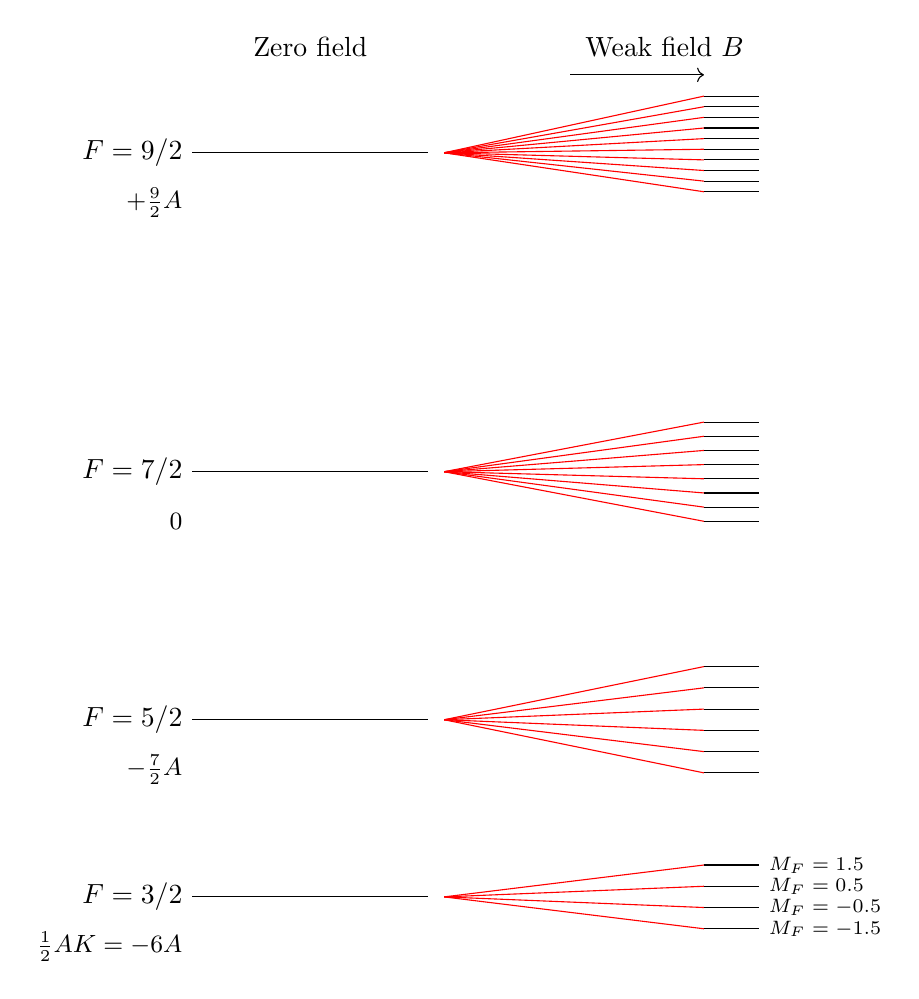
\begin{tikzpicture}[xscale=1.0,yscale=0.9]
    % zero-field levels on left
    \draw (0,-6) -- (3,-6); \node[left] at (0,-6) {$F=3/2$};
    \draw (0,-3.5) -- (3,-3.5); \node[left] at (0,-3.5) {$F=5/2$};
    \draw (0,0) -- (3,0); \node[left] at (0,0) {$F=7/2$};
    \draw (0,4.5) -- (3,4.5); \node[left] at (0,4.5) {$F=9/2$};
    \node[left] at (0,-6.7) {\small$\tfrac12 AK=-6A$};
    \node[left] at (0,-4.2) {\small$-\tfrac72 A$};
    \node[left] at (0,-0.7) {\small$0$};
    \node[left] at (0,3.8) {\small$+\tfrac92 A$};

    % Zeeman fan out for each
    % F=3/2 -> 4 lines
    \foreach \m/\y in {-1.5/-6.45,-0.5/-6.15,0.5/-5.85,1.5/-5.55}{
        \draw[red] (3.2,-6) -- (6.5,\y);
        \draw (6.5,\y) -- (7.2,\y);
        \node[right] at (7.2,\y) {\scriptsize $M_F=\m$};
    }
    % F=5/2 -> 6 lines
    \foreach \m/\y in {-2.5/-4.25,-1.5/-3.95,-0.5/-3.65,0.5/-3.35,1.5/-3.05,2.5/-2.75}{
        \draw[red] (3.2,-3.5) -- (6.5,\y);
        \draw (6.5,\y) -- (7.2,\y);
    }
    % F=7/2 -> 8 lines
    \foreach \m/\y in {-3.5/-0.7,-2.5/-0.5,-1.5/-0.3,-0.5/-0.1,0.5/0.1,1.5/0.3,2.5/0.5,3.5/0.7}{
        \draw[red] (3.2,0) -- (6.5,\y);
        \draw (6.5,\y) -- (7.2,\y);
    }
    % F=9/2 -> 10 lines
    \foreach \m/\y in {-4.5/3.95,-3.5/4.1,-2.5/4.25,-1.5/4.4,-0.5/4.55,0.5/4.7,1.5/4.85,2.5/5.0,3.5/5.15,4.5/5.3}{
        \draw[red] (3.2,4.5) -- (6.5,\y);
        \draw (6.5,\y) -- (7.2,\y);
    }
    \node at (1.5,6) {Zero field};
    \node at (6,6) {Weak field $B$};
    \draw[->] (4.8,5.6) -- (6.5,5.6);
\end{tikzpicture}
\end{center}
Sublevel spacing within an $F$ manifold is $g_F\mu_B B$ and differs between manifolds because $g_F$ depends on $F$.

\subsection*{(e) Strong field for $1s\,{}^2S_{1/2}$ of hydrogen}

In the strong-field regime the hyperfine term $A\vec I\cdot\vec J$ is the perturbation; $J_z$, $I_z$ become good quantum numbers. For hydrogen $J=S=1/2$, $I=1/2$, with $g_J\to g_s$ and $g_I\to g_p$. To first order,
\begin{equation*}
    \Delta E(M_J,M_I) = g_s\mu_B B\,M_J - g_p\mu_N B\,M_I + A\,M_J M_I\,\hbar^2,
\end{equation*}
where we henceforth absorb $\hbar^2$ into $A$. The four states $\ket{M_J,M_I}$ with $M_J,M_I=\pm 1/2$ give:

\begin{center}
\begin{tabular}{@{}ccc@{}}\toprule
$(M_J,M_I)$ & $\Delta E$ \\ \midrule
$(+\tfrac12,+\tfrac12)$ & $\tfrac12 g_s\mu_B B-\tfrac12 g_p\mu_N B+\tfrac14 A$ \\
$(+\tfrac12,-\tfrac12)$ & $\tfrac12 g_s\mu_B B+\tfrac12 g_p\mu_N B-\tfrac14 A$ \\
$(-\tfrac12,+\tfrac12)$ & $-\tfrac12 g_s\mu_B B-\tfrac12 g_p\mu_N B-\tfrac14 A$ \\
$(-\tfrac12,-\tfrac12)$ & $-\tfrac12 g_s\mu_B B+\tfrac12 g_p\mu_N B+\tfrac14 A$ \\
\bottomrule
\end{tabular}
\end{center}

% --- verify the stated ratio ---
Numerator of the required ratio:
\begin{align*}
    \Delta E_{+,-}+\Delta E_{-,-} &= \left(\tfrac12 g_s\mu_B B+\tfrac12 g_p\mu_N B-\tfrac14 A\right) + \left(-\tfrac12 g_s\mu_B B+\tfrac12 g_p\mu_N B+\tfrac14 A\right) \\
    &= g_p\mu_N B.
\end{align*}
Denominator:
\begin{align*}
    \Delta E_{+,-}+\Delta E_{+,+} &= \left(\tfrac12 g_s\mu_B B+\tfrac12 g_p\mu_N B-\tfrac14 A\right) + \left(\tfrac12 g_s\mu_B B-\tfrac12 g_p\mu_N B+\tfrac14 A\right) \\
    &= g_s\mu_B B.
\end{align*}
Dividing,
\begin{equation*}
    \boxed{\;\frac{\Delta E_{J_z=1/2,I_z=-1/2}+\Delta E_{J_z=-1/2,I_z=-1/2}}{\Delta E_{J_z=1/2,I_z=-1/2}+\Delta E_{J_z=1/2,I_z=1/2}} = \frac{g_p\mu_N}{g_s\mu_B}.\;}
\end{equation*}
The numerator isolates the \emph{nuclear} Zeeman coupling (electronic contributions cancel for opposite $M_J$) while the denominator isolates the \emph{electronic} Zeeman coupling, yielding the ratio of the two magnetic moments.

%==========================================================================
\section*{Question 4 --- Semi-classical atom--field interaction}
%==========================================================================

\subsection*{(a) Coupled amplitude equations}

Write the state as a superposition of unperturbed eigenstates:
\begin{equation*}
    \Psi(\vec r,t) = c_1(t)\,\psi_1(\vec r)\,e^{-iE_1 t/\hbar} + c_2(t)\,\psi_2(\vec r)\,e^{-iE_2 t/\hbar}.
\end{equation*}
Substituting into the TDSE $i\hbar\partial_t\Psi = (H_0+V)\Psi$ and using $H_0\psi_n=E_n\psi_n$ leaves
\begin{equation*}
    i\hbar\bigl[\dot c_1\psi_1 e^{-iE_1t/\hbar}+\dot c_2\psi_2 e^{-iE_2t/\hbar}\bigr] = V(t)\bigl[c_1\psi_1 e^{-iE_1t/\hbar}+c_2\psi_2 e^{-iE_2t/\hbar}\bigr].
\end{equation*}
Project onto $\psi_1^*$ (using orthonormality) and onto $\psi_2^*$:
\begin{equation*}
    i\hbar\dot c_1 = c_2\,V_{12}(t)\,e^{-i\omega_0 t},\qquad i\hbar\dot c_2 = c_1\,V_{21}(t)\,e^{+i\omega_0 t},
\end{equation*}
where $\omega_0=(E_2-E_1)/\hbar$ and $V_{ab}(t)=\int\psi_a^* V(t)\psi_b\,d\vec r$. For $V(t)=exE_0\cos(\omega t)$ we have $V_{ab}(t)=E_0\cos(\omega t)\int\psi_a^*(ex)\psi_b\,d\vec r = -E_0\cos(\omega t)\,\chi_{ab}$ using the definition $\chi_{ab}=-e\!\int\psi_a^* x\psi_b\,d\vec r$.

Writing $\cos(\omega t)=\tfrac12(e^{i\omega t}+e^{-i\omega t})$ and substituting,
\begin{equation}
\boxed{\;
\begin{aligned}
    \dot c_1(t) &= \frac{iE_0\chi_{12}}{2\hbar}\bigl[e^{i(\omega-\omega_0)t}+e^{-i(\omega+\omega_0)t}\bigr]\,c_2(t), \\
    \dot c_2(t) &= \frac{iE_0\chi_{12}}{2\hbar}\bigl[e^{-i(\omega-\omega_0)t}+e^{i(\omega+\omega_0)t}\bigr]\,c_1(t),
\end{aligned}\;}\label{eq:coupled}
\end{equation}
using $\chi_{21}=\chi_{12}^*=\chi_{12}$ (real for real bound-state wavefunctions and the operator $x$).

\subsection*{(b) Weak-field solution with the rotating-wave approximation}

Initial conditions $c_1(0)=1$, $c_2(0)=0$. For a weak perturbation take $c_1(t)\approx 1$ throughout. The second equation reads
\begin{equation*}
    \dot c_2(t) = \frac{iE_0\chi_{12}}{2\hbar}\left[e^{-i(\omega-\omega_0)t}+e^{i(\omega+\omega_0)t}\right].
\end{equation*}
Near resonance $|\omega-\omega_0|\ll\omega+\omega_0$, so the second term oscillates rapidly at $\omega+\omega_0\sim 2\omega$ and averages to zero: this is the \emph{rotating-wave approximation} (RWA). Dropping it and integrating from $0$ to $t$,
\begin{equation*}
    c_2(t) = \frac{iE_0\chi_{12}}{2\hbar}\int_0^t e^{-i(\omega-\omega_0)t'}dt' = \frac{iE_0\chi_{12}}{2\hbar}\cdot\frac{e^{-i(\omega-\omega_0)t}-1}{-i(\omega-\omega_0)}.
\end{equation*}
Hence
\begin{equation}
    \boxed{\;|c_2(t)|^2 = \frac{E_0^2\chi_{12}^2}{\hbar^2}\,\frac{\sin^2\!\bigl[(\omega-\omega_0)t/2\bigr]}{(\omega-\omega_0)^2}.\;}\label{eq:c2sq}
\end{equation}

\subsection*{(c) Einstein $B_{12}$ coefficient}

The field is now broadband. Replace $E_0^2$ in \eqref{eq:c2sq} by its spectral content: the radiation energy density in the interval $d\omega$ is
\begin{equation*}
    dU = \tfrac12\varepsilon_0 E_0^2(\omega)\,d\omega = u(\omega)\,d\omega \;\Longrightarrow\; E_0^2(\omega)\,d\omega = \frac{2u(\omega)}{\varepsilon_0}d\omega,
\end{equation*}
and the upper-state probability sums incoherently over spectral components,
\begin{equation*}
    |c_2(t)|^2 = \int\frac{2\chi_{12}^2\,u(\omega)}{\varepsilon_0\hbar^2}\,\frac{\sin^2[(\omega-\omega_0)t/2]}{(\omega-\omega_0)^2}\,d\omega.
\end{equation*}
The sinc-squared kernel, as a function of $\omega$, is sharply peaked at $\omega=\omega_0$ for large $t$. Using
\begin{equation*}
    \lim_{t\to\infty}\frac{\sin^2[(\omega-\omega_0)t/2]}{(\omega-\omega_0)^2} = \frac{\pi t}{2}\,\delta(\omega-\omega_0),
\end{equation*}
and assuming $u(\omega)$ varies slowly over the width of the kernel (i.e.\ broad spectrum),
\begin{equation*}
    |c_2(t)|^2 = \frac{\pi\chi_{12}^2}{\varepsilon_0\hbar^2}\,u(\omega_0)\,t.
\end{equation*}
The transition rate is $d|c_2|^2/dt\equiv B_{12}\,u(\omega_0)/3$ once isotropic radiation is averaged (the factor $1/3$ comes from $\overline{\cos^2\theta}=1/3$ when averaging the dipole--field angle), giving
\begin{equation}
    \boxed{\;B_{12} = \frac{\pi\,\chi_{12}^2}{3\varepsilon_0\hbar^2}.\;}\label{eq:B12}
\end{equation}

\subsection*{(d) $B_{12}$ for hydrogen $1s\to 2p$}

We need $\chi_{12}^2$ summed over the degenerate final $2p$ sublevels (the $2p$ manifold has $m=0,\pm1$).

% --- angular reduction ---
Write $x=r\sin\theta\cos\phi$. With the tabulated spherical harmonics,
\begin{equation*}
    Y_{1,-1}-Y_{1,+1} = \sqrt{\frac{3}{8\pi}}\,\sin\theta\,(e^{-i\phi}+e^{+i\phi}) = 2\sqrt{\frac{3}{8\pi}}\,\sin\theta\cos\phi,
\end{equation*}
so
\begin{equation*}
    x = r\sin\theta\cos\phi = r\sqrt{\frac{2\pi}{3}}\bigl(Y_{1,-1}-Y_{1,+1}\bigr).
\end{equation*}
The matrix element decomposes as $\chi_{1s\to 2p,m}=-e\,I_r\cdot A_m$ with
\begin{equation*}
    I_r = \int_0^\infty R_{10}(r)\,r\,R_{21}(r)\,r^2\,dr, \qquad A_m = \sqrt{\frac{2\pi}{3}}\!\int Y_{0,0}^*\bigl(Y_{1,-1}-Y_{1,+1}\bigr)Y_{1,m}\,d\Omega.
\end{equation*}

% --- angular integrals ---
Using $Y_{0,0}=1/\sqrt{4\pi}$ and orthonormality $\int Y_{\ell,m'}^*Y_{\ell,m}d\Omega=\delta_{m',m}$, together with $Y_{\ell,-m}=(-1)^m Y_{\ell,m}^*$:
\begin{equation*}
    A_0 = 0,\qquad A_{+1} = \sqrt{\frac{2\pi}{3}}\cdot\frac{1}{\sqrt{4\pi}}\cdot(-1) = -\frac{1}{\sqrt{6}},\qquad A_{-1} = \sqrt{\frac{2\pi}{3}}\cdot\frac{1}{\sqrt{4\pi}}\cdot(+1) = +\frac{1}{\sqrt{6}}.
\end{equation*}
Thus only $m=\pm 1$ contribute and
\begin{equation*}
    \sum_m |A_m|^2 = \frac{1}{6}+\frac{1}{6}=\frac{1}{3}.
\end{equation*}

% --- radial integral ---
From the table: $R_{10}=2 a_0^{-3/2}e^{-r/a_0}$ and $R_{21}=(2/\sqrt{3})a_0^{-3/2}(r/2a_0)e^{-r/2a_0}=(1/\sqrt{3})a_0^{-5/2}r\,e^{-r/2a_0}$. Hence
\begin{align*}
    I_r &= \int_0^\infty\!\! 2a_0^{-3/2}e^{-r/a_0}\,\cdot\,\frac{1}{\sqrt{3}}a_0^{-5/2}r\,e^{-r/2a_0}\,\cdot r^3\,dr \\
    &= \frac{2}{\sqrt{3}}\,a_0^{-4}\int_0^\infty r^4\,e^{-3r/(2a_0)}\,dr \\
    &= \frac{2}{\sqrt{3}}\,a_0^{-4}\cdot\frac{4!}{(3/2a_0)^5} = \frac{2}{\sqrt{3}}\cdot 24\cdot\frac{2^5}{3^5}\,a_0 = \frac{2^{8}\cdot\sqrt{3}}{3^{5}}\,a_0 = \frac{256\sqrt{3}}{243}\,a_0.
\end{align*}
(Equivalently $I_r = (2^{15/2}/3^{5})\,a_0\approx 1.290\,a_0\cdot\sqrt{8}\approx 3.65\,a_0$.)

% --- combine ---
Summing over the three $2p$ sublevels,
\begin{equation*}
    \sum_m \chi_{1s\to 2p,m}^2 = e^2\,I_r^2\,\sum_m |A_m|^2 = e^2\cdot\frac{256^2\cdot 3}{243^2}a_0^2\cdot\frac{1}{3} = \left(\frac{256}{243}\right)^{2}\!\cdot e^2 a_0^2\cdot\frac{3\cdot 3}{3}.
\end{equation*}
Let me collect this carefully: $I_r^2 = (256\sqrt{3}/243)^2 a_0^2 = (256^2\cdot 3/243^2)a_0^2$. Multiplying by $\sum_m|A_m|^2=1/3$:
\begin{equation*}
    \sum_m\chi_{1s,2p_m}^2 = e^2 a_0^2\cdot\frac{256^2\cdot 3}{243^2}\cdot\frac{1}{3} = e^2 a_0^2\left(\frac{256}{243}\right)^2 = e^2 a_0^2\cdot\frac{65536}{59049}.
\end{equation*}
Numerically $(256/243)^2\approx 1.110$, so $\chi_{12}^2\approx 1.110\,e^2 a_0^2$ (where $\chi_{12}^2$ denotes the sum over degenerate final states). Substituting in \eqref{eq:B12}:
\begin{equation*}
    B_{12} = \frac{\pi}{3\varepsilon_0\hbar^2}\cdot\left(\frac{256}{243}\right)^2 e^2 a_0^2.
\end{equation*}

Inserting numerical values
($e=1.602\times10^{-19}\,\text{C}$, $a_0=5.292\times10^{-11}\,\text{m}$, $\varepsilon_0=8.854\times10^{-12}\,\text{F\,m}^{-1}$, $\hbar=1.055\times10^{-34}\,\text{J\,s}$):
\begin{equation*}
    \frac{e^2 a_0^2}{\varepsilon_0\hbar^2} = \frac{(1.602\times10^{-19})^2(5.292\times10^{-11})^2}{(8.854\times10^{-12})(1.055\times10^{-34})^2}
    \approx 7.29\times10^{20}\ \text{m}^3\,\text{J}^{-1}\,\text{s}^{-2},
\end{equation*}
giving
\begin{equation*}
    \boxed{\;B_{12}^{\,1s\to 2p}=\frac{\pi}{3}\cdot\left(\frac{256}{243}\right)^2\cdot 7.29\times10^{20}\;\text{m}^3\text{J}^{-1}\text{s}^{-2}\approx 8.5\times 10^{20}\;\text{m}^3\text{J}^{-1}\text{s}^{-2}.\;}
\end{equation*}
(Equivalently, expressed per unit frequency rather than per unit angular frequency, $B_{12}^{(\nu)}=2\pi B_{12}^{(\omega)}\approx 5.3\times 10^{21}\,\text{m}^3\text{J}^{-1}\text{s}^{-2}$.)

\end{document}
